\documentclass[12pt]{article}
\usepackage[a4paper,left=27mm,right=27mm,top=24mm,bottom=22mm]{geometry}
\usepackage[space]{ctex}
\usepackage{graphicx}
\usepackage{float}
\usepackage{subfigure}
\usepackage{amsmath}
\usepackage{amsfonts,amssymb}
\title{\LARGE\textbf{Learning Neutral Network}}
\author{SA21010060 周俊亦}
\date{}

\begin{document}
	\maketitle
	\renewcommand{\abstractname}{Abstract}
	\begin{abstract}
		神经网络的本质在于函数拟合。神经网络基本的结构由非线性变化单元组成,具有很强的非线性映射能力,理论上 BP 神经网络算法可以逼近任意函数。借助于这一点,目前,神经网络算法在众多领域的应用都取得了可观的成就,如自然语言处理、图像理解等。本次作业学习神经网络方法,分别对 mnist 数据集、昆虫数据集、平面数据集、以及 fashion-mnist 数据集实现图像分类。
	\end{abstract}
	
	\section{实验平台}
	
	本次作业的所有实验全部基于 python 的神经网络库 PyTorch 编写。
	
	\section{神经网络介绍}
	
	人工神经网络(artificial neural network,ANN),简称神经网络(neural network,NN), 是一种模仿生物神经网络的结构和功能的数学模型或计算模型。
	
	\begin{figure}[H]
		\centering
		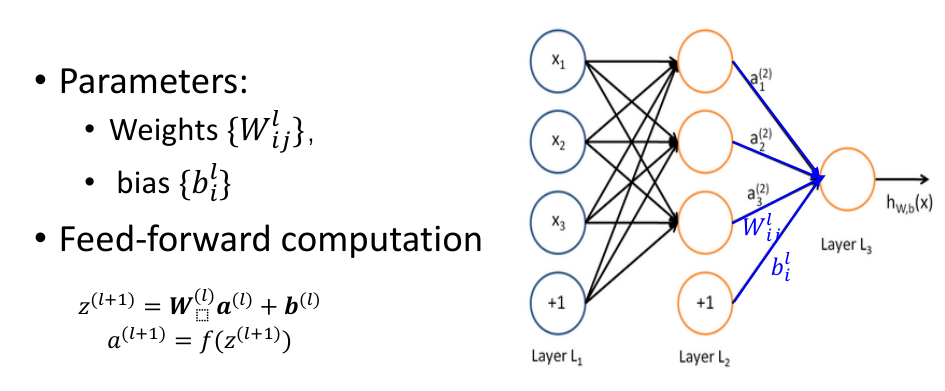
\includegraphics[width=6in]{./images/nn_model.png}
		\centering
		\caption{神经网络}
	\end{figure}
	
	神经网络由大量的节点(或称“神经元”)和之间相互的联接构成。每个节点输出经过一种特定的函数变换,称为激活函数(activation function)。每两个节点间的联接都代表一个对于通过该连接信号的加权值,称之为权重。
	
	总而言之,通过节点,神经网络将具有特征维度的输入数据转换成了具有特征维度的输出数据,神经网络可以通过调整网络权值来改变这种转换关系。事实上,神经网络的应用正是诞生在了这种从输入到输出的转换关系上。神经网络的魅力在于它能根据需求,通过适当的设计,自主的去寻找这种转换关系,而无需人类的干预,在数学上,这叫做函数拟合。因此,我们说,神经网络的本质是函数拟合。
	
	\section{MNIST}
	
	\subsection{介绍}
	
	MNIST手写数字数据集是深度学习中的经典数据集,该数据集中的数字图片是由250个不同职业的人手写绘制的,其中训练集数据一共60000张图片,测试集数据一共10000张图片。每张手写数字图片大小都是28*28,每张图片代表的是从0到9中的每个数字。
	
	数据集样例如下所示:
	
	\begin{figure}[H]
		\centering
		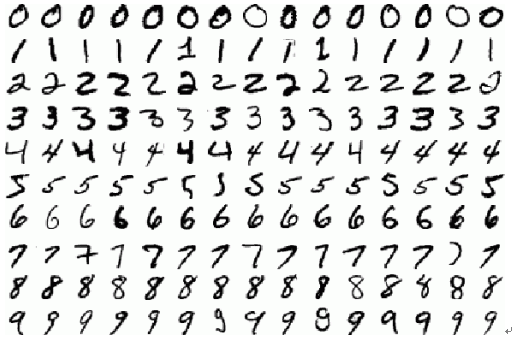
\includegraphics[width=4.5in]{./images/mnistexample.png}
		\centering
		\caption{MNIST}
	\end{figure}
	
	\subsection{网络训练分析}
	
	\subsubsection{混淆矩阵}
	
	在机器学习中,混淆矩阵 (Confusion Matrix) 是一种非常好的可视化结果工具。在图像精度评价中,主要用于比较分类结果和实际测得值。
	
	混淆矩阵的每一列代表了预测类别,每一列的总数表示预测为该类别的数据的数目;每一行代表了数据的真实归属类别,每一行的数据总数表示该类别的数据实例的数目。
	
	\subsubsection{训练分析}
	实验搭建神经网络训练模型进行图片分类训练。自行搭建三层卷积神经网络,设计时考虑每层的参数数目尽量一致,设计神经网络结构如下:
	
	\begin{figure}[H]
		\centering
		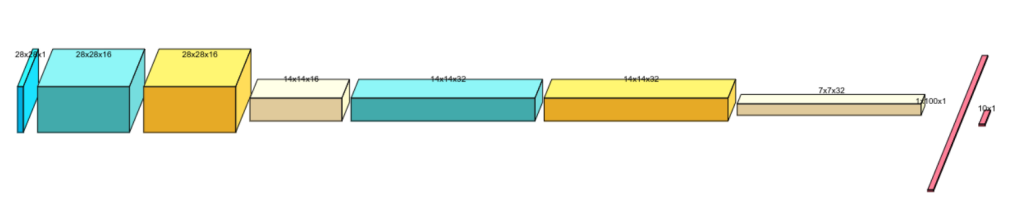
\includegraphics[width=6in]{./images/mnist_network.png}
		\centering
		\caption{网络结构}
	\end{figure}
	
	设置批样本数量 BATCHSIZE = 128, epoch = 20 的情况下,调整学习率进行网络性能分析,结果如下:
	
	\begin{figure}[H]
		\centering
		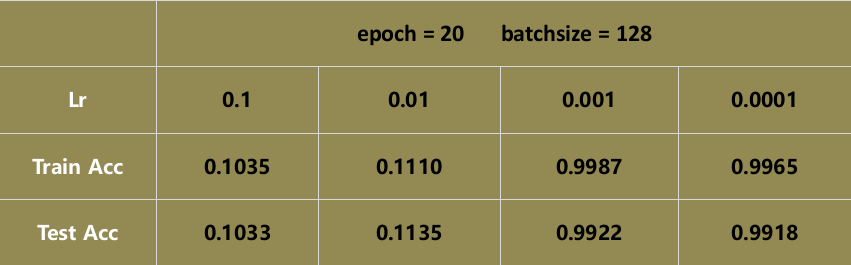
\includegraphics[width=4.5in]{./images/mnist_train.png}
		\centering
		\caption{分组性能对比}
	\end{figure}
	
	在学习率为 LR = 0.1 和 LR = 0.01 的情况下,在训练中发现损失函数一直处于较高位,且准确率一直在低位徘徊,推测是由于学习率较大使得梯度下降过程中无法收敛。
	

	减小学习率至 LR = 0.001,网络成功收敛,在迭代 20 轮后在训练集和测试集上都达到了 $99\%$ 的准确率。
	
	
	\begin{figure}[H]
		\centering
		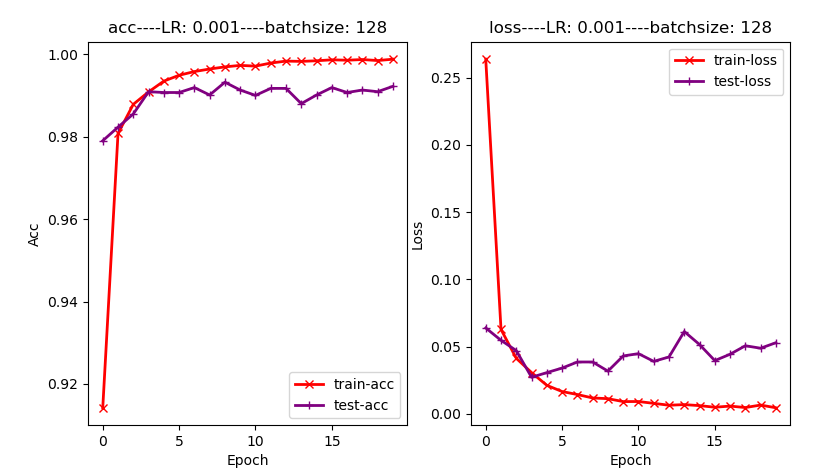
\includegraphics[width=4.2in]{./images/mnist_loss.png}
		\centering
		\caption{loss曲线}
	\end{figure}
	
	\begin{figure}[H]
		\centering
		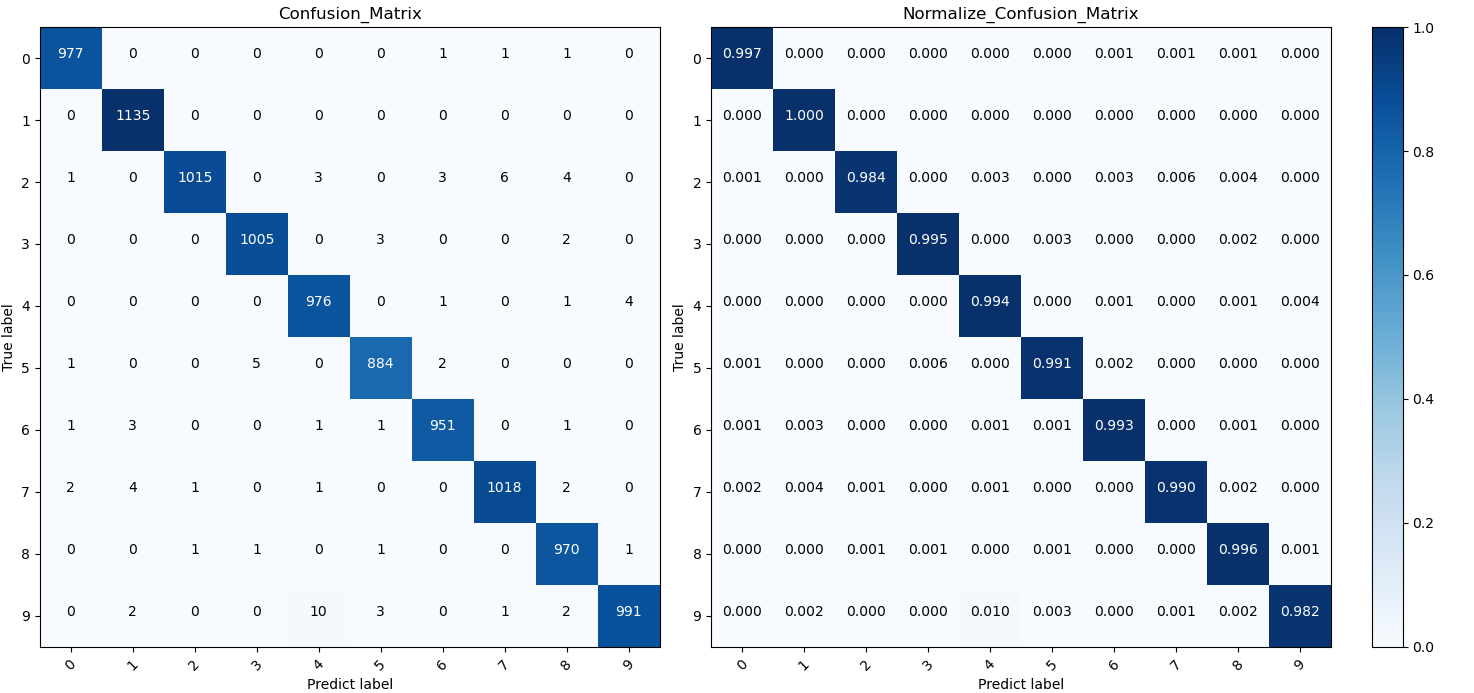
\includegraphics[width=5.5in]{./images/mnist_confusion.png}
		\centering
		\caption{训练结果-混淆矩阵}
	\end{figure}
	
	从混淆矩阵可以看出,MNIST 数据集的手写数字样本数量并不是均分的。
	
	选取分类错误案例进行查看。例如:查看混淆矩阵第五行的最后一列,可以看到数字 4 有四个被错误的预测成了数字 9, 查看具体图片如下:
	
	\begin{figure}[H]
		\centering
		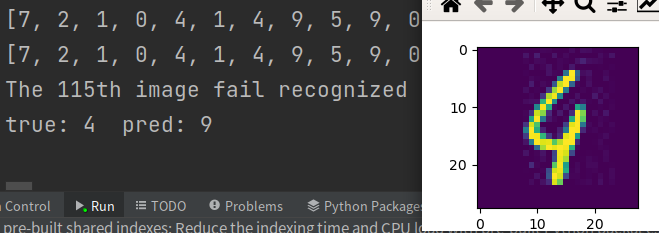
\includegraphics[width=5in]{./images/fail_ex.png}
		\centering
		\caption{分类错误案例}
	\end{figure}
	
	可以看出,这个数字 4 写得确实像 9,分类错误在一定程度上可以理解。这也说明 MNIST 数据集有一定的噪声。
	
	
	\section{昆虫分类}
	
	\textbf{样本描述}:生物学家对某昆虫进行研究,发现该昆虫具有3个不同的属性,即可分为3类,依据的资料是体长和翼长。
	
	数据格式为:每一行 (x,y,label):x为体长值,y为翼长值,label为所属类别0/1/2

	
	\subsection{不带噪声的昆虫数据集}
	
	训练集样本分布:三个不同的颜色点分别表示不同种类的昆虫
	
	\begin{figure}[H]
		\centering
		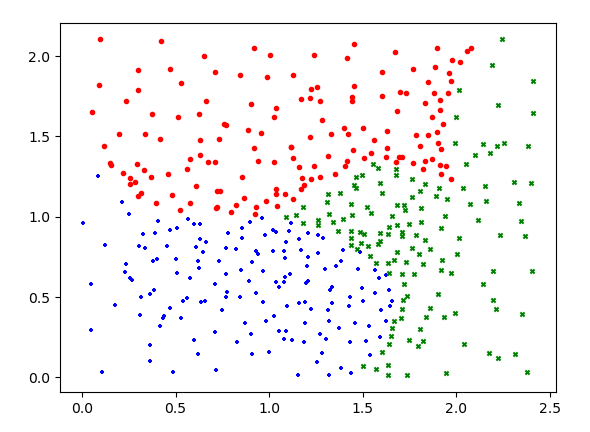
\includegraphics[width=3.3in]{./images/insects_normal_train_dist.png}
		\centering
		\caption{训练集样本分布}
	\end{figure}
	
	由于样本集的数据量少,特征简单,故设计简单的含两层隐藏层的网络进行训练,设计两层隐藏层的目的是避免样本特征的真实函数含有阶跃信号而导致拟合不够准确。当神经网络小于两层时,只能逼近不含阶跃信号的函数。
	
	选取 BATCHSIZE = 4, EPOCH = 300, 选取不同学习率后,结果如下:
	
	\begin{figure}[H]
		\centering
		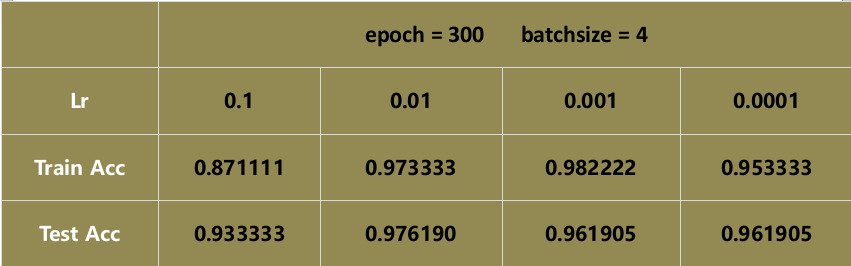
\includegraphics[width=4in]{./images/insects_normal_train.png}
		\centering
		\caption{训练结果}
	\end{figure}
	
	查看损失函数曲线如下:
	
	\begin{figure}[H]
		\centering
		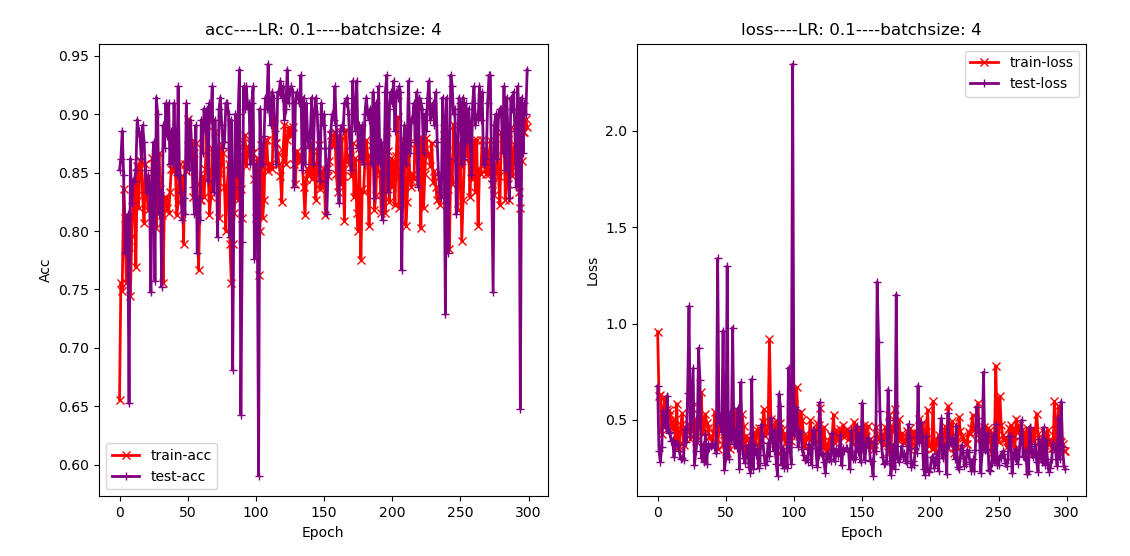
\includegraphics[width=5in]{./images/insects_normal_loss01.png}
		\centering
		\caption{LR = 0.1}
	\end{figure}

	\begin{figure}[H]
		\centering
		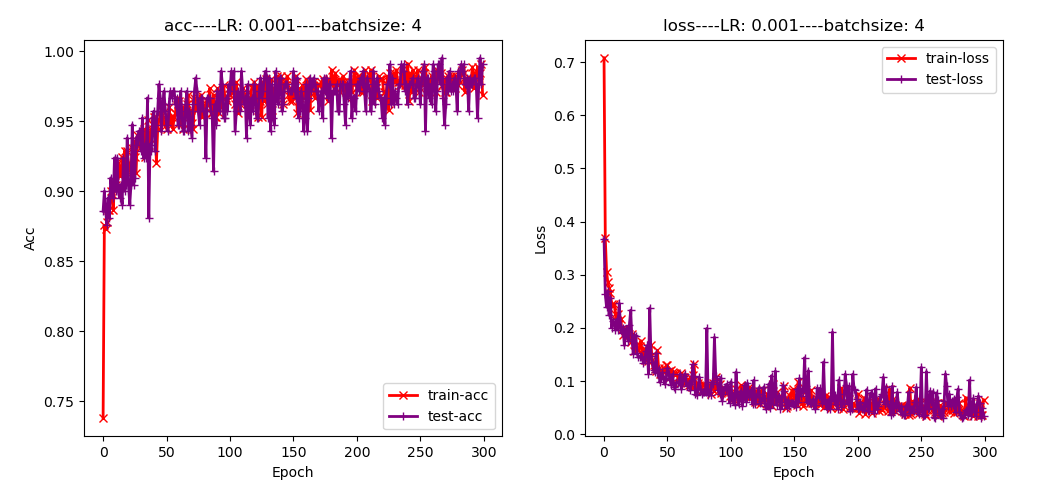
\includegraphics[width=4.7in]{./images/insects_normal_loss0001.png}
		\centering
		\caption{LR = 0.001}
	\end{figure}
	
	\begin{figure}[H]
		\centering
		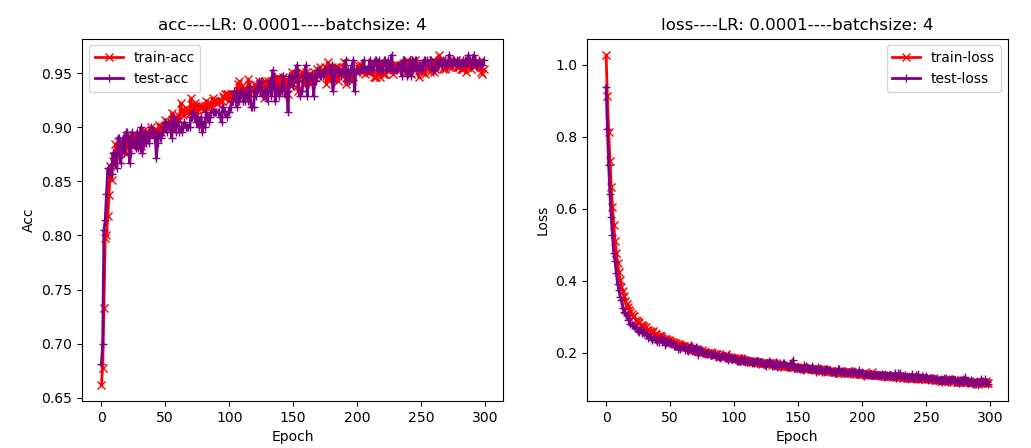
\includegraphics[width=4.7in]{./images/insects_normal_loss00001.png}
		\centering
		\caption{LR = 0.0001}
	\end{figure}
	
	可以发现,除了 LR = 0.1 外,其他学习率都收敛到了较好的准确率。在此例中,学习率越小,误差曲线更平滑。但是准确率并没有越来越高,于是进行\textbf{动态调整学习率}实验。
	
	动态调整学习率设置为初始 LR = 0.01, 之后分别在第 50 个 EPOCH 将学习率变为原来的 0.1 倍,在第 150 个 EPOCH 将学习率继续变为原来的 0.1 倍,之后不再改变,结果如下:
	
	\begin{figure}[H]
		\centering
		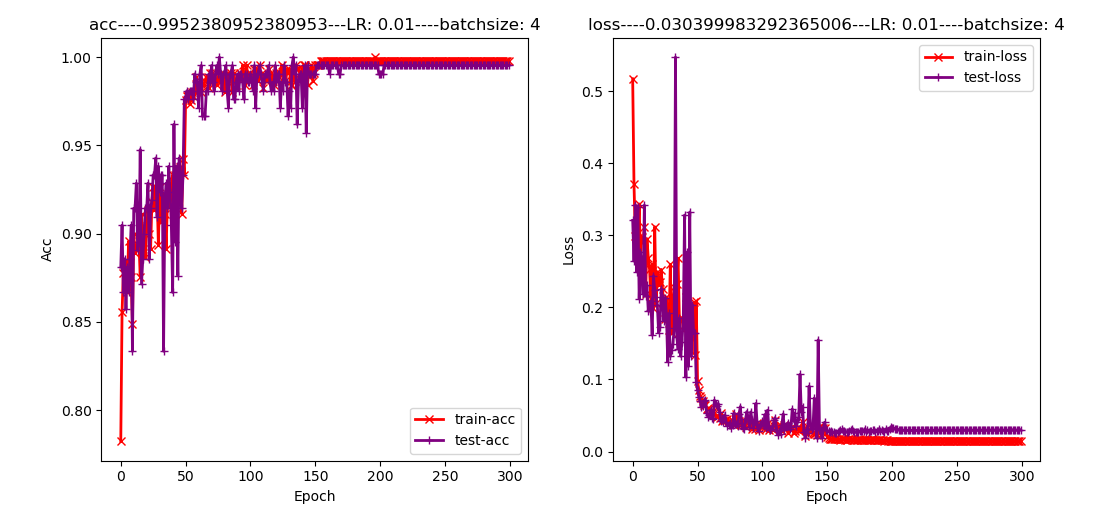
\includegraphics[width=4.5in]{./images/insects_normal_loss_step.png}
		\centering
		\caption{动态调整LR(比固定学习率效果要好)}
	\end{figure}
	
	300 个 EPOCH 后,训练集准确率为 0.997778, 测试集准确率为 0.995238,结果比之前都要好!从曲线形状可以看出,准确率曲线在前 70 轮借助于大学习率快速下降,而后借助于学习率调整而趋于平稳。
	
	查看分类结果如下,其中左侧是训练集分布,右侧是测试集的预测结果,红绿蓝色分别表示预测正确的各类点,黑色三角点为分类错误点,可以看到,仅只有一个分类错误点(在右图右上角)。
	
	\begin{figure}[H]
		\centering
		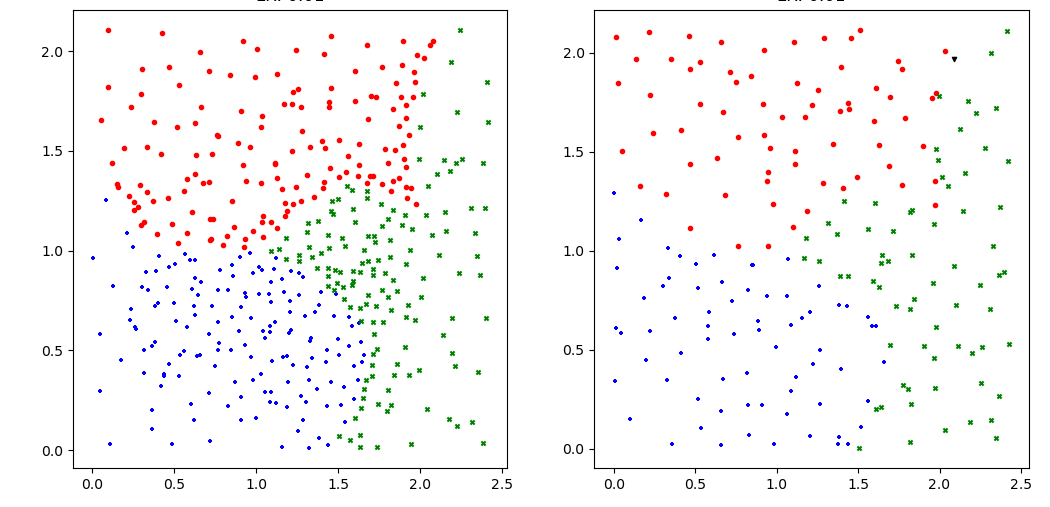
\includegraphics[width=5.7in]{./images/insects_normal_result.png}
		\centering
		\caption{分类结果}
	\end{figure}
	
	混淆矩阵如下:
	
	\begin{figure}[H]
		\centering
		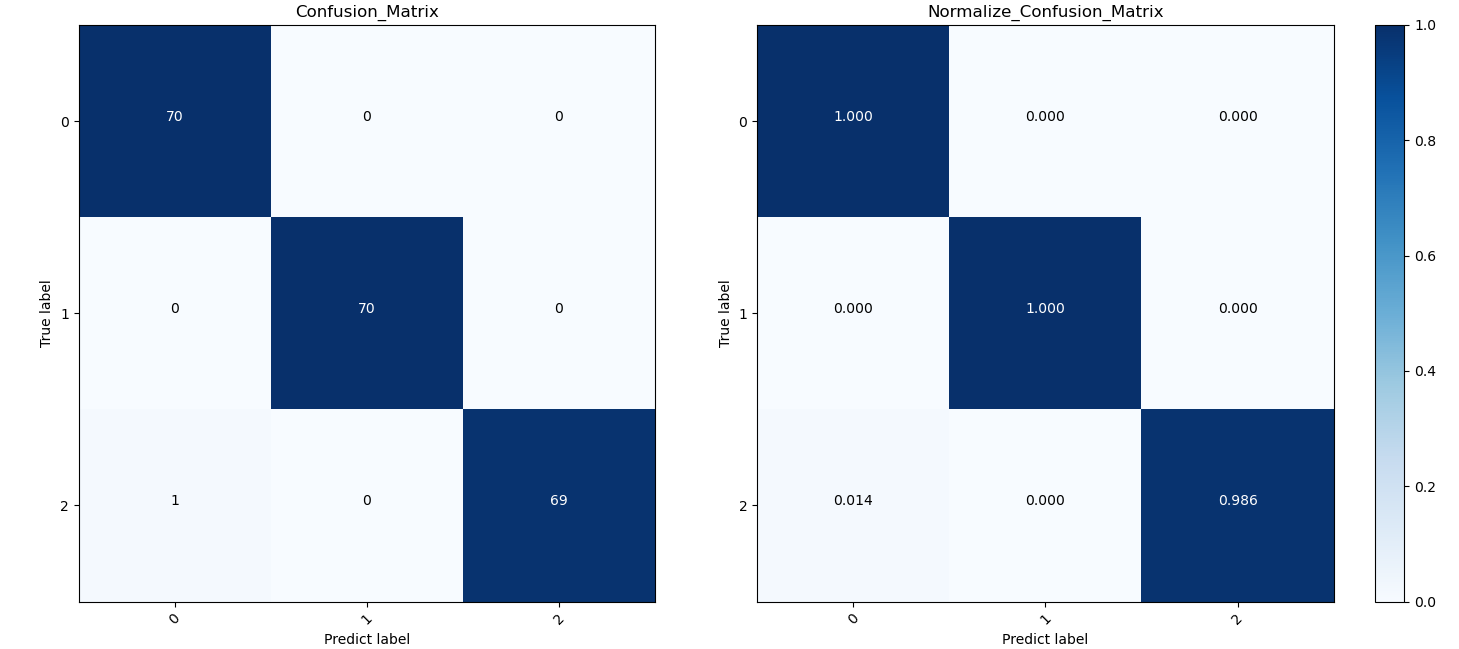
\includegraphics[width=5.7in]{./images/insects_normal_confusion.png}
		\centering
		\caption{混淆矩阵}
	\end{figure}

	\subsection{带噪声的昆虫数据集}
	
	从上一例可以看出,动态学习率调整对网络训练有较好的效果,因此,接下来,我们直接使用动态学习率调整的网络训练。
	
	\begin{figure}[H]
		\centering
		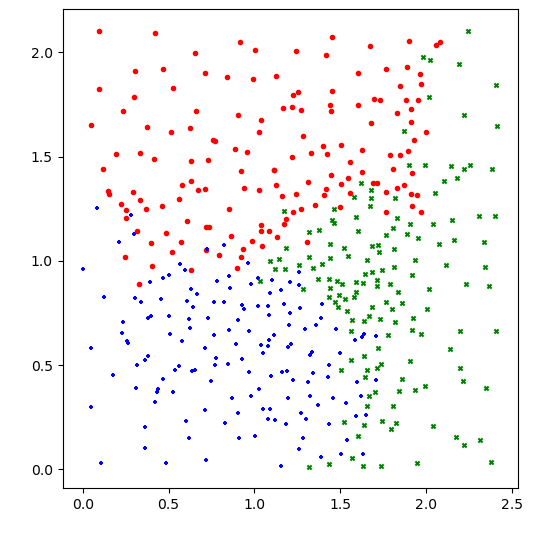
\includegraphics[width=3in]{./images/insects_noise_train_dist.png}
		\centering
		\caption{带噪声的训练集样本分布}
	\end{figure}
	
	可以看到,训练集的点云边界有点类交错,说明带有了噪声。
	
	使用动态调整学习率策略,迭代 600 个 EPOCH 后结果如下:
	
	\begin{figure}[H]
		\centering
		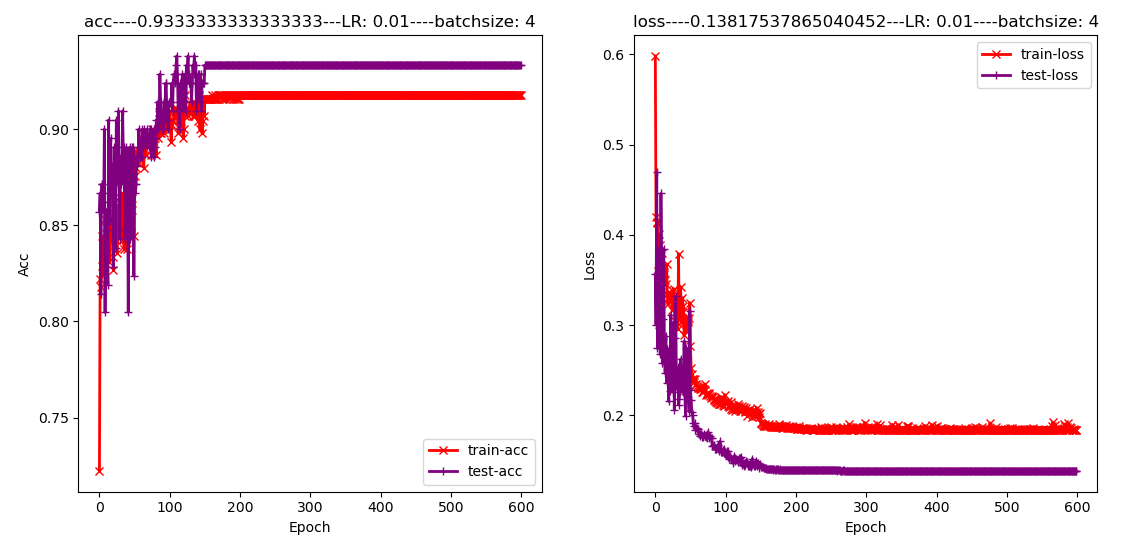
\includegraphics[width=5in]{./images/insects_noise_loss_step.png}
		\centering
		\caption{动态调整LR}
	\end{figure}
	
	600 个 EPOCH 后,训练集准确率为 0.922222, 测试集准确率为 0.933333,结果比不带噪声的数据要差。
	
	查看分类结果如下,其中左侧是训练集分布,右侧是测试集的预测结果,红绿蓝色分别表示预测正确的各类点,黑色三角点为分类错误点,可以看到,边界点分类错误居多。
	
	\begin{figure}[H]
		\centering
		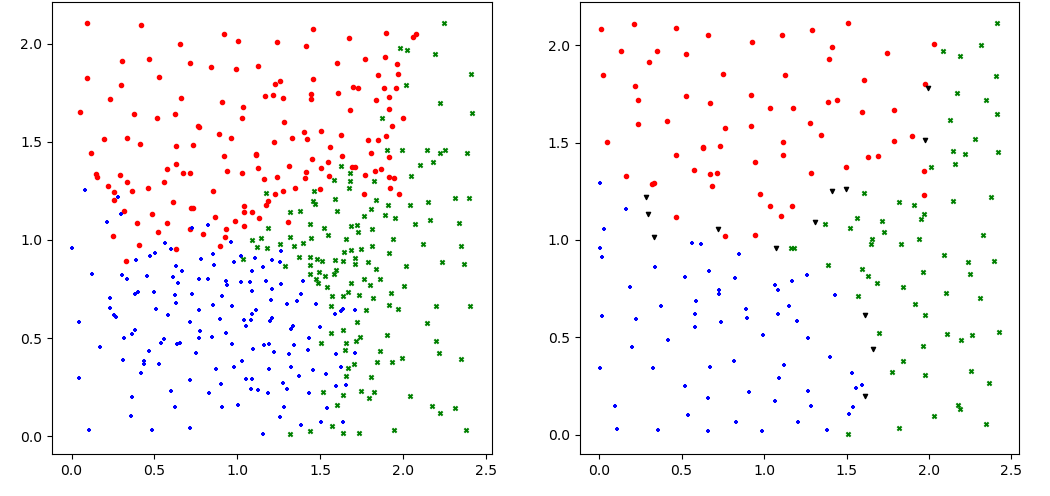
\includegraphics[width=5.7in]{./images/insects_noise_result.png}
		\centering
		\caption{分类结果}
	\end{figure}
	
	混淆矩阵如下:
	
	\begin{figure}[H]
		\centering
		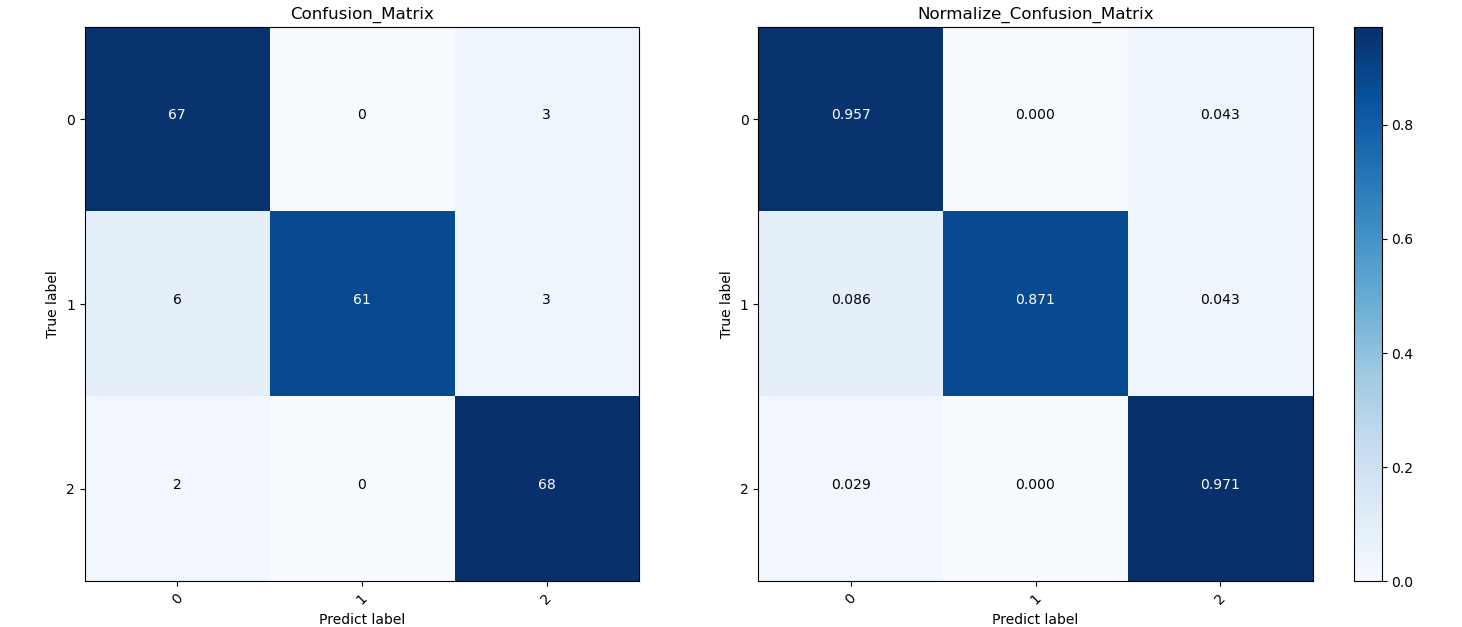
\includegraphics[width=5.7in]{./images/insects_noise_confusion.png}
		\centering
		\caption{混淆矩阵}
	\end{figure}
	
	\subsection{带噪声与不带噪声的昆虫数据集训练结果对比}
	
	带噪声与不带噪声的昆虫数据集训练结果对比如下图,同样迭代 500 个 epoch 后,在不带噪声数据集上训练和测试的准确率比带噪声的要高,这是符合逻辑的。同时,观察收敛情况,不带噪声数据集上训练,在第 100 个 epoch 附近已经几乎收敛了,但是在噪声数据集上训练,接近第 170 左右 epoch 才几乎收敛。
	
	\begin{figure}[H]
		\centering
		\subfigure[normal]{
			\begin{minipage}[t]{0.9\linewidth}
				\centering
				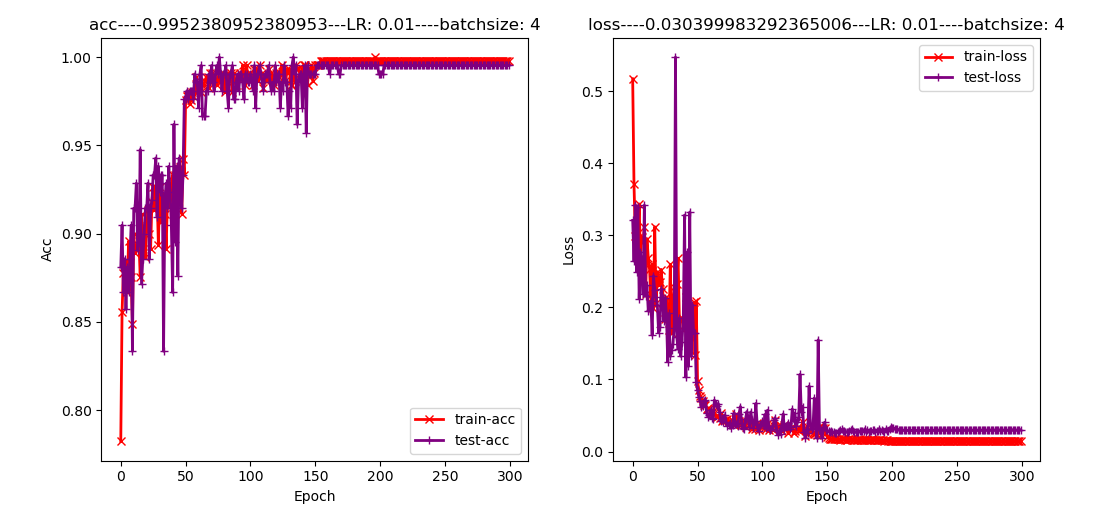
\includegraphics[width=4in]{./images/insects_normal_loss_step.png}
				%\caption{fig1}
			\end{minipage}%
		}%
		
		\subfigure[noise]{
			\begin{minipage}[t]{0.9\linewidth}
				\centering
				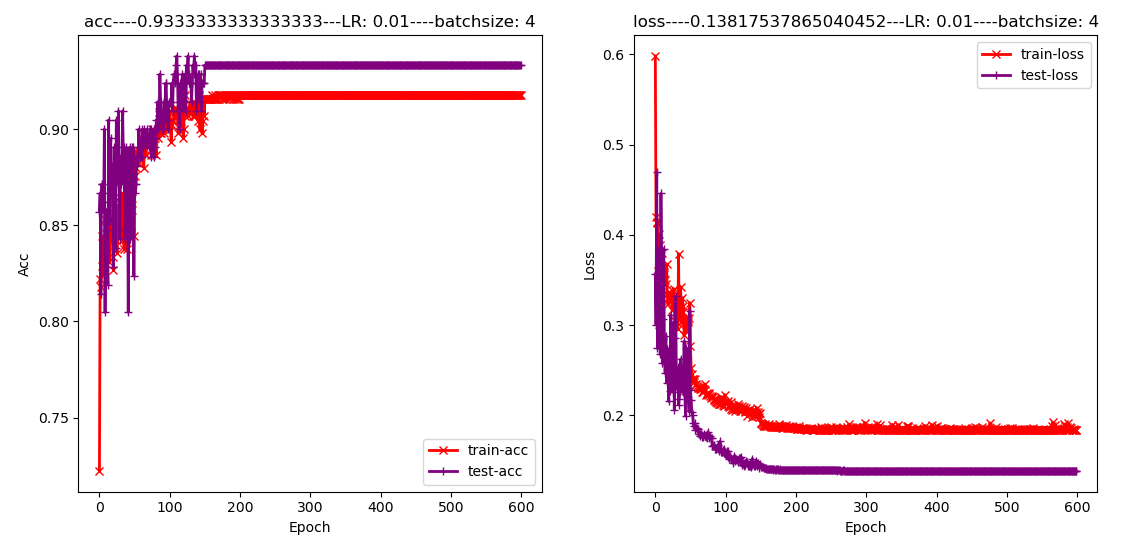
\includegraphics[width=4in]{./images/insects_noise_loss_step.png}
				%\caption{fig2}
			\end{minipage}%
		}
		\centering
		\caption{训练结果对比}
	\end{figure}
	
	\subsection{选取不同激活函数结果对比}
	
	在不带噪声的昆虫数据集下,采用不同激活函数的结果如下:
	
	\begin{figure}[H]
		\centering
		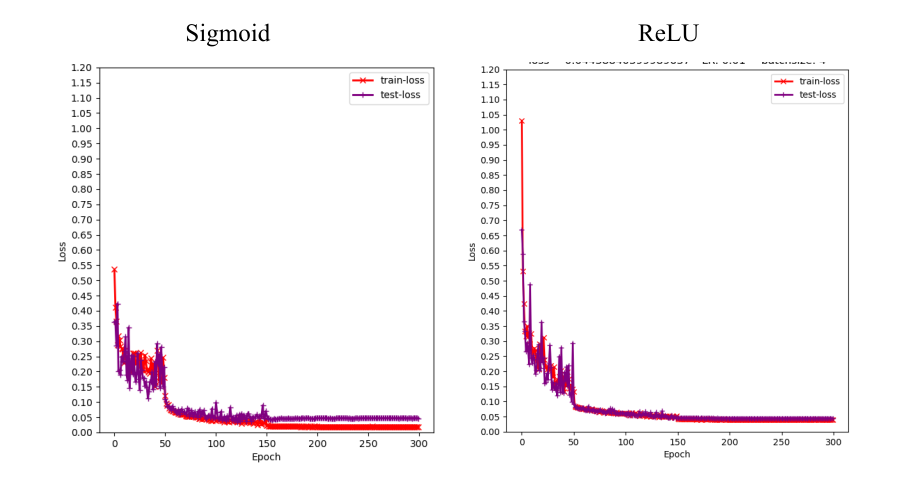
\includegraphics[width=4.5in]{./images/insects_sigmoid_relu.png}
		\centering
		\caption{训练集样本分布}
	\end{figure}
	
	理论上,在深度分类网络上使用 Sigmoid 容易出现梯度消失情况,在本例中,没有观察到明显区别。
	
	\section{平面点集分类}
	
	平面点集结构与昆虫数据集类似,分为了 20 类点,数据集总量比昆虫数据集要大。因此,在昆虫网络的基础上稍微调整了隐藏层神经元个数,提升了参数数量。
	
	
	\subsection{不带噪声的平面点数据集}
	
	训练集样本分布:二十个不同的颜色点分别表示不同种类的点
	
	\begin{figure}[H]
		\centering
		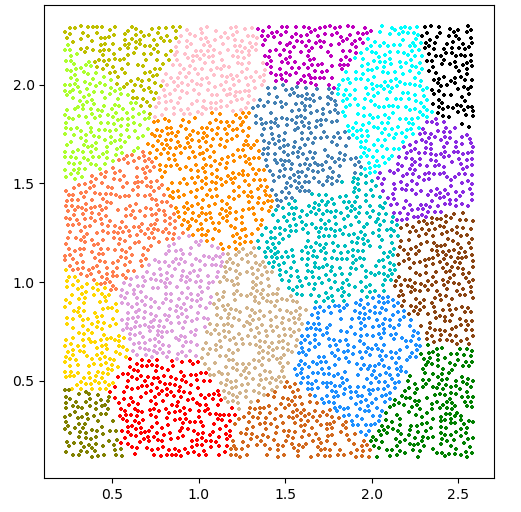
\includegraphics[width=2in]{./images/plane_normal_train_dist.png}
		\centering
		\caption{训练集样本分布}
	\end{figure}
	
	使用动态调整学习率策略,迭代 500 个 EPOCH 后, 训练集准确率为 0.992998,测试集准确率为 0.981019,损失曲线结果如下:
	
	\begin{figure}[H]
		\centering
		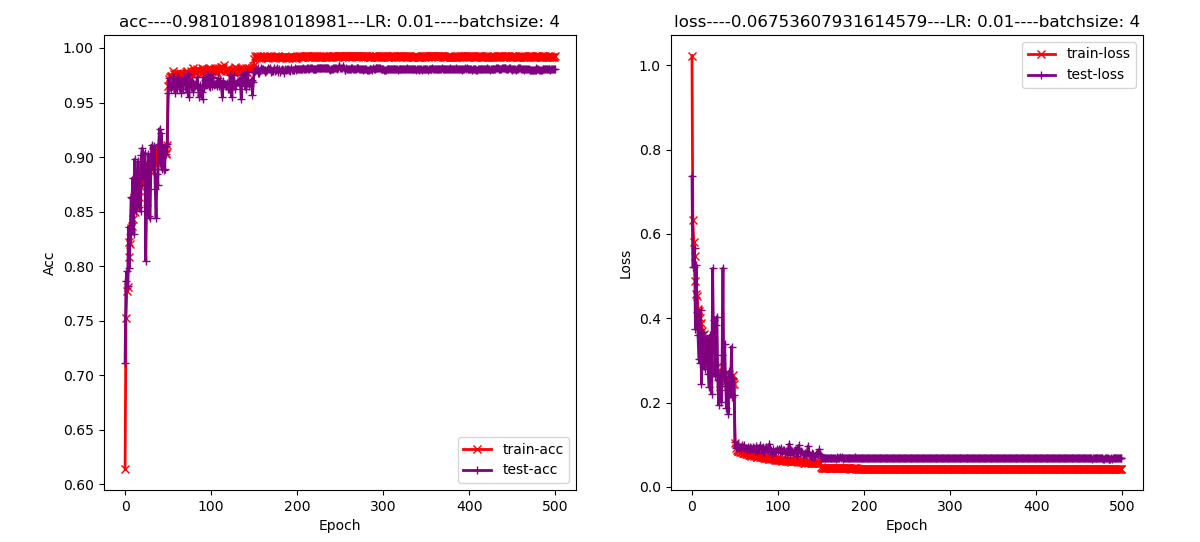
\includegraphics[width=4.5in]{./images/plane_normal_loss_step.png}
		\centering
		\caption{动态调整LR}
	\end{figure}

	查看分类结果如下,不同颜色分别表示预测正确的各类点,黑色三角点为分类错误点,可以看到,分类错误边界点居多。
	
	\begin{figure}[H]
		\centering
		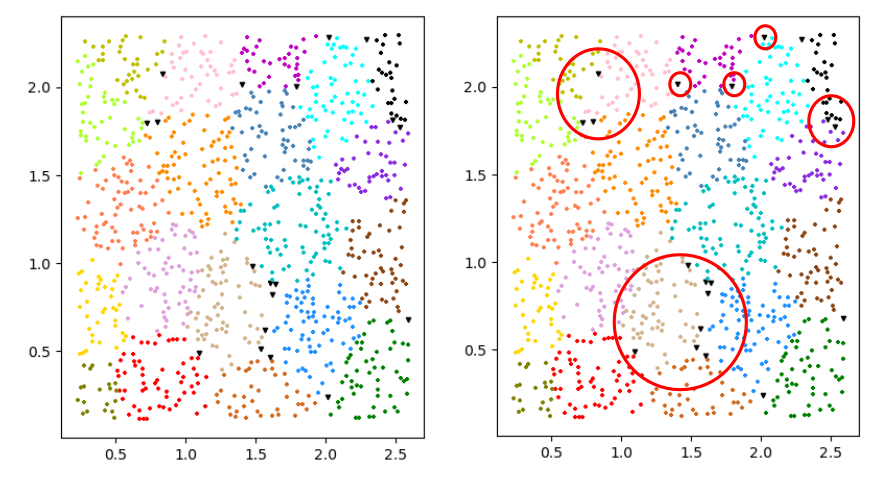
\includegraphics[width=4.2in]{./images/plane_normal_result.png}
		\centering
		\caption{分类结果}
	\end{figure}

	混淆矩阵如下:
	
	\begin{figure}[H]
		\centering
		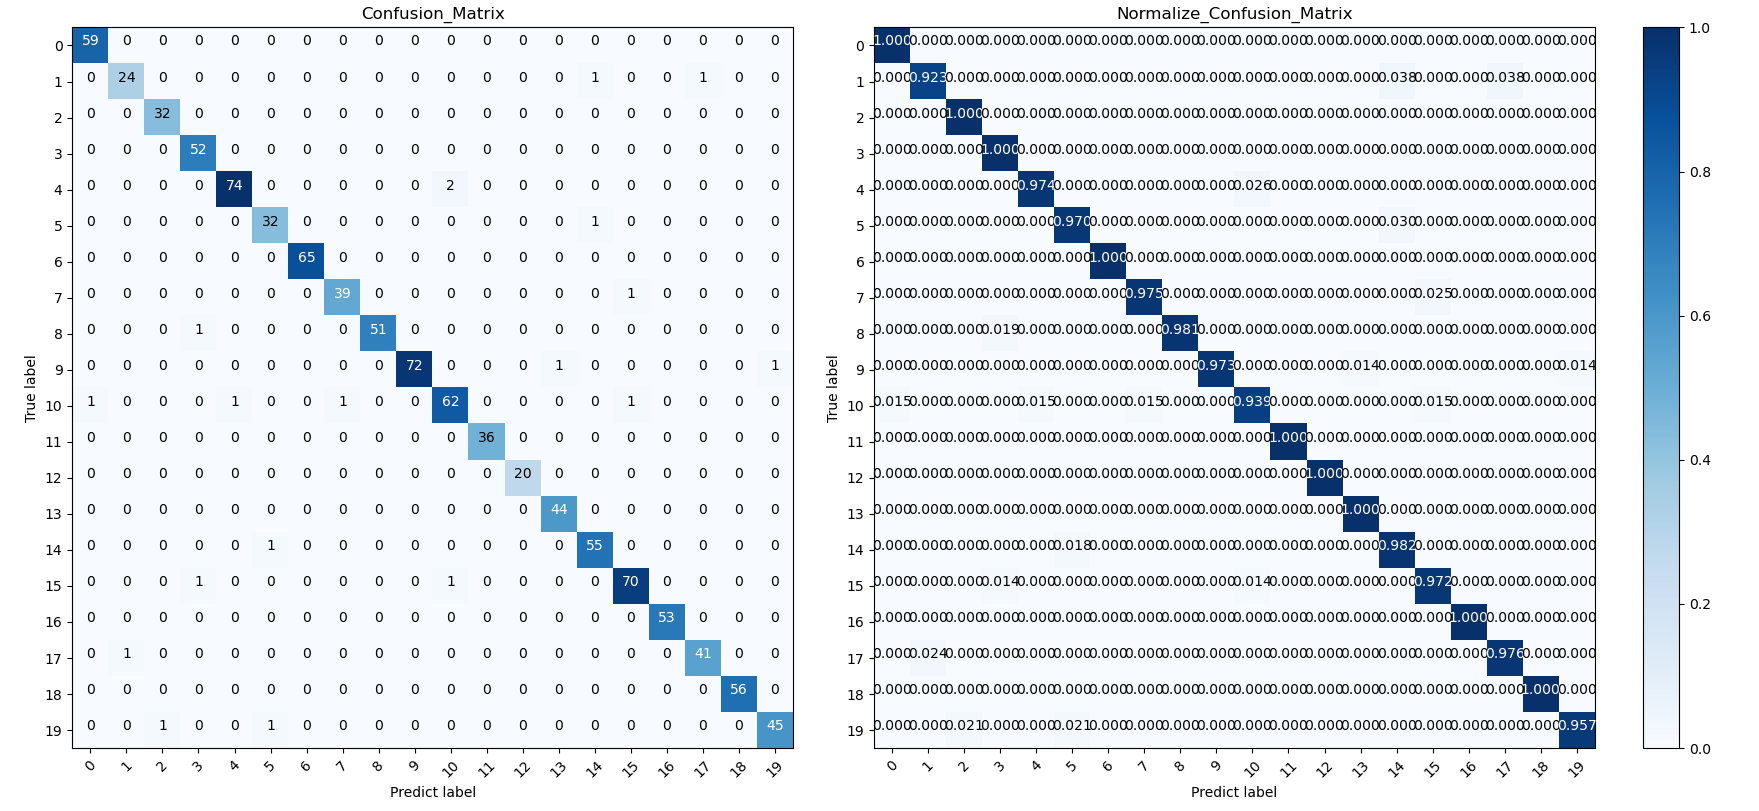
\includegraphics[width=4.6in]{./images/plane_normal_confusion.png}
		\centering
		\caption{混淆矩阵}
	\end{figure}
	
	\subsection{带噪声的平面点数据集}
	
	训练集样本分布:二十个不同的颜色点分别表示不同种类的点,训练集的点云边界有点类交错,说明带有噪声。
	
	\begin{figure}[H]
		\centering
		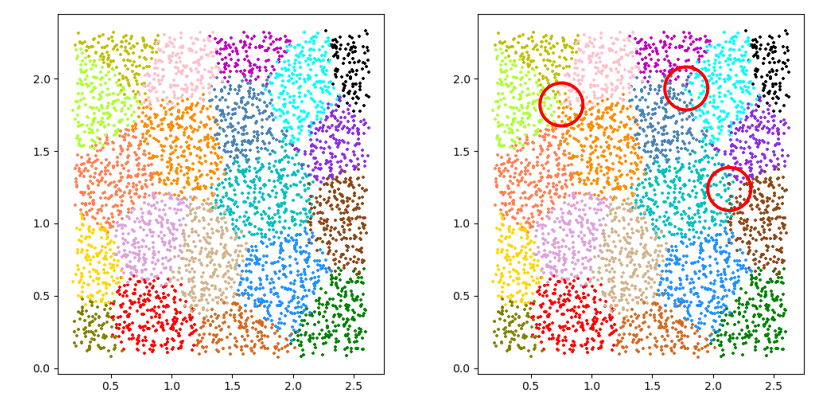
\includegraphics[width=3.8in]{./images/plane_noise_train_dist.png}
		\centering
		\caption{训练集样本分布}
	\end{figure}

	使用动态调整学习率策略,迭代 500 个 EPOCH 后, 训练集准确率为 0.938985,测试集准确率为 0.932068,损失曲线结果如下:
	
	\begin{figure}[H]
		\centering
		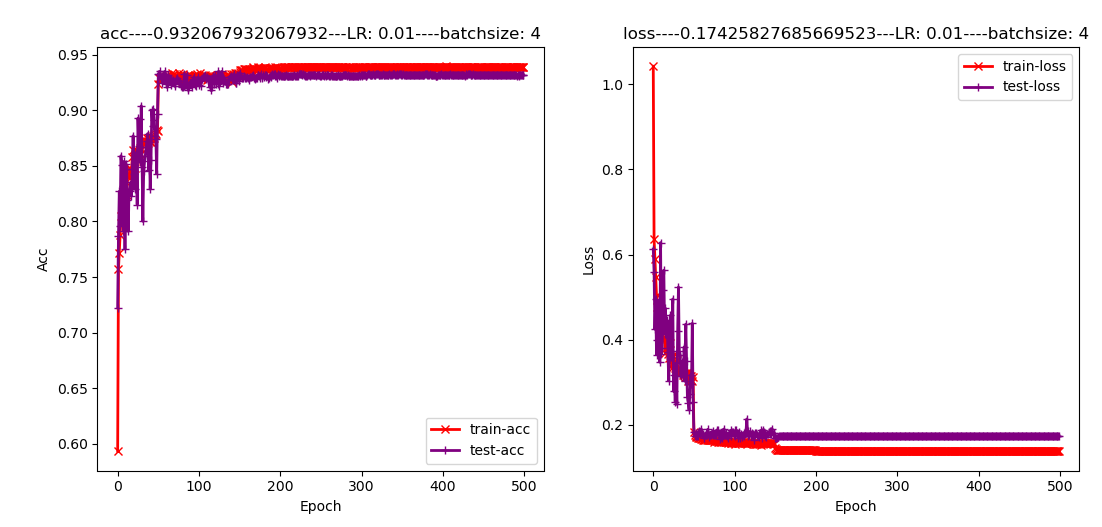
\includegraphics[width=4in]{./images/plane_noise_loss_step.png}
		\centering
		\caption{动态调整LR}
	\end{figure}

	查看分类结果如下,不同颜色分别表示预测正确的各类点,黑色三角点为分类错误点,可以看到,分类错误边界点居多。
	
	\begin{figure}[H]
		\centering
		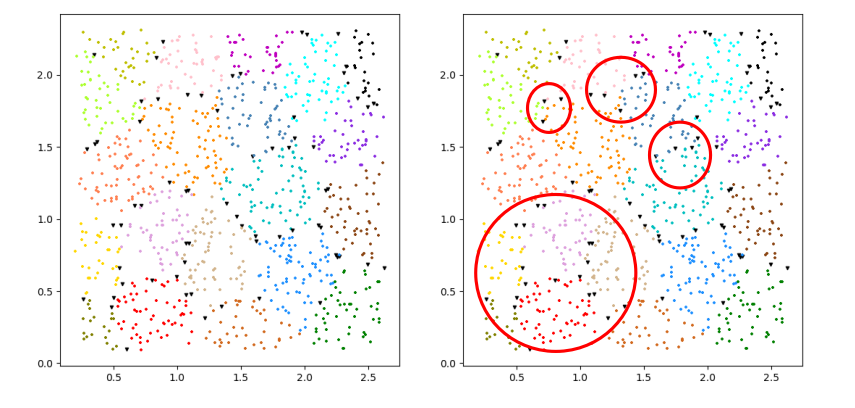
\includegraphics[width=3.8in]{./images/plane_noise_result.png}
		\centering
		\caption{分类结果}
	\end{figure}

	混淆矩阵如下:
	
	\begin{figure}[H]
		\centering
		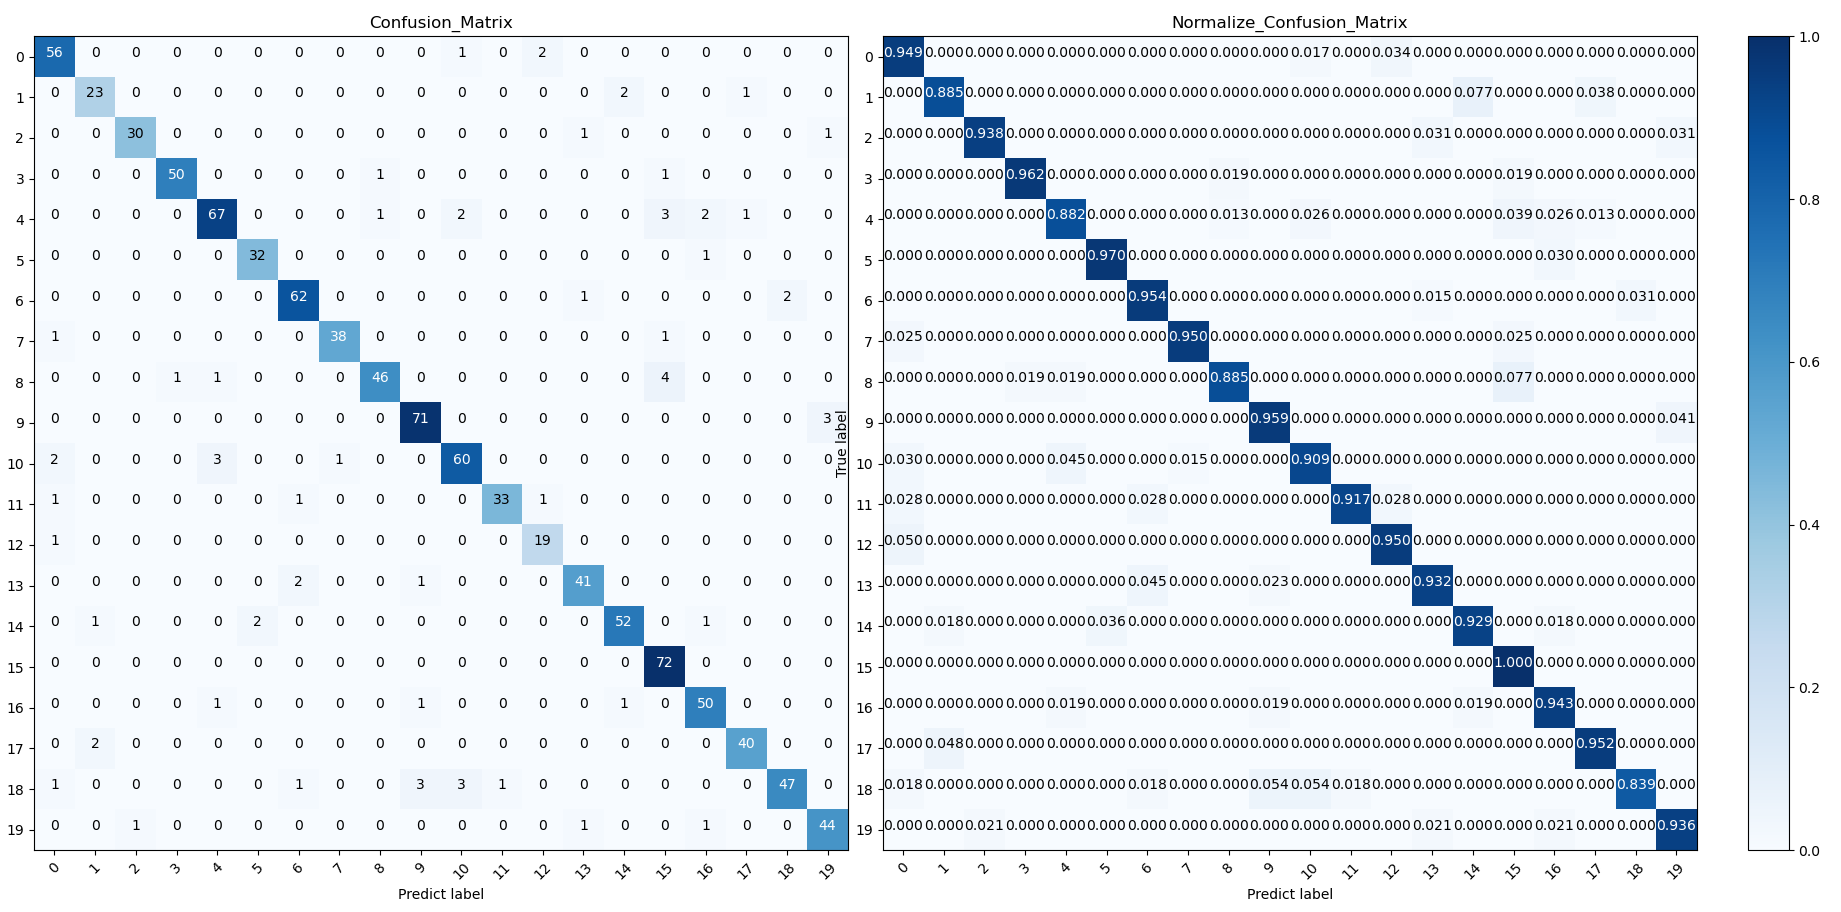
\includegraphics[width=4.6in]{./images/plane_noise_confusion.png}
		\centering
		\caption{混淆矩阵}
	\end{figure}
	
	
	
	\section{Fashion-MNIST 数据集}
	
	\subsection{介绍}
	
	如第一个实验所述,经典的MNIST数据集包含了大量的手写数字。十几年来,来自机器学习、机器视觉、人工智能、深度学习领域的研究员们把这个数据集作为衡量算法的基准之一。
	
	但是,经过近些年来的发展,MNIST 数据集已经不能满足算法验证的需要,原因如下:
	
	\begin{itemize}
		\item MNIST太简单了。很多深度学习算法在测试集上的准确率已经达到$99.6\%$(在第一次作业就连笔者随意搭建的一个简单卷积网络在测试集上的准确率都达到了$99\%$)。
		\item MNIST数字识别的任务不能代表现代机器学习的主要需求。在 MNIST 上看似有效的想法没有办法迁移到真正的机器视觉问题上。
	\end{itemize}
	
	此时,Fashion-MNIST 应运而生。Fashion-MNIST是一个替代MNIST手写数字集的图像数据集。 它是由Zalando(一家德国的时尚科技公司)旗下的研究部门提供。其涵盖了来自10种类别的共7万个不同商品的正面图片(都是服饰鞋类,比简单的手写数字要难得多)。Fashion-MNIST的大小、格式和训练集/测试集划分与原始的MNIST完全一致。60000/10000的训练测试数据划分,28x28的灰度图片。
	
	数据集样例如下所示:
	
	\begin{figure}[H]
		\centering
		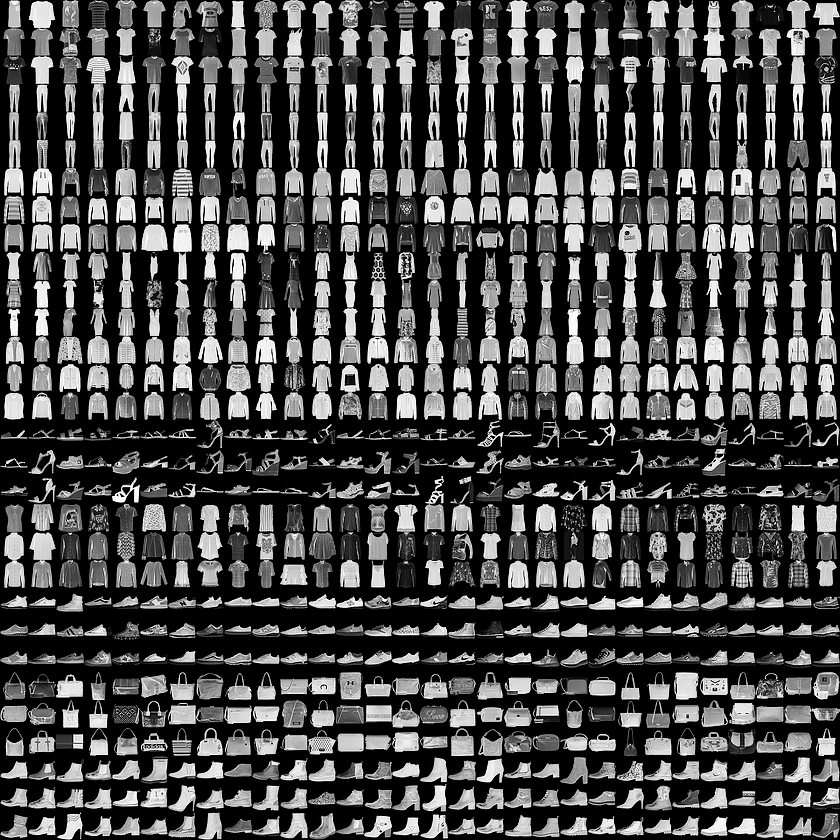
\includegraphics[width=4in]{./images/fashion_example.png}
		\centering
		\caption{Fashion-MNIST}
	\end{figure}
	
	\subsection{网络训练分析}
	
	使用与 MNIST 相同的三层卷积神经网络进行训练,采用动态学习率调整方法,每迭代 10 个 EPOCH 学习率调整为原来的 0.1 倍,初值取 LR = 0.01 ,  BATCHSIZE = 128 ,STEP = 10,实验结果如下:
	
	\begin{figure}[H]
		\centering
		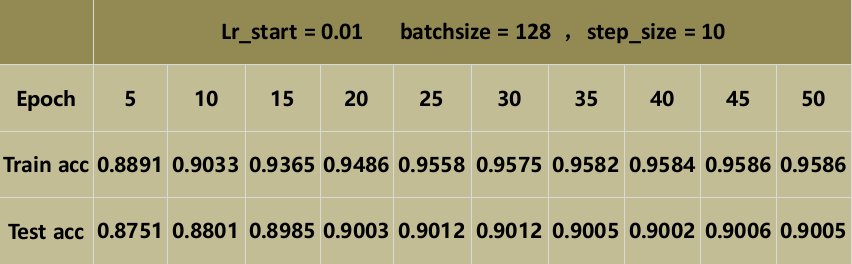
\includegraphics[width=6in]{./images/fashion1.png}
		\centering
		\caption{LR = 0.01 BATCHSIZE = 128 STEP = 10}
	\end{figure}

	观察发现,到了训练集正确率为0.95左右,即 epoch = 25左右,正确率上升十分缓慢,测试集正确率甚至出现降低,说明在此时遇到了瓶颈,或者是过拟合,可能是学习率在此时太低所导致,遂以固定lr分组测试。结果如下:
	
	\begin{figure}[H]
		\centering
		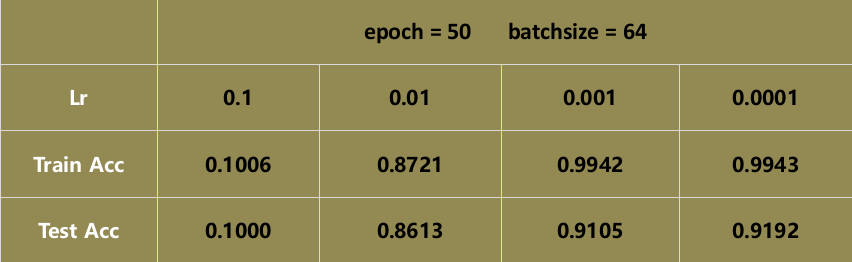
\includegraphics[width=6in]{./images/fashion2.png}
		\centering
		\caption{LR 分组}
	\end{figure}
	
	损失曲线如下,可以看到均存在过拟合现象,LR = 0.001 时在测试集准确率最好。
	
	\begin{figure}[H]
		\centering
		\subfigure[LR = 0.1]{
			\begin{minipage}[t]{0.5\linewidth}
				\centering
				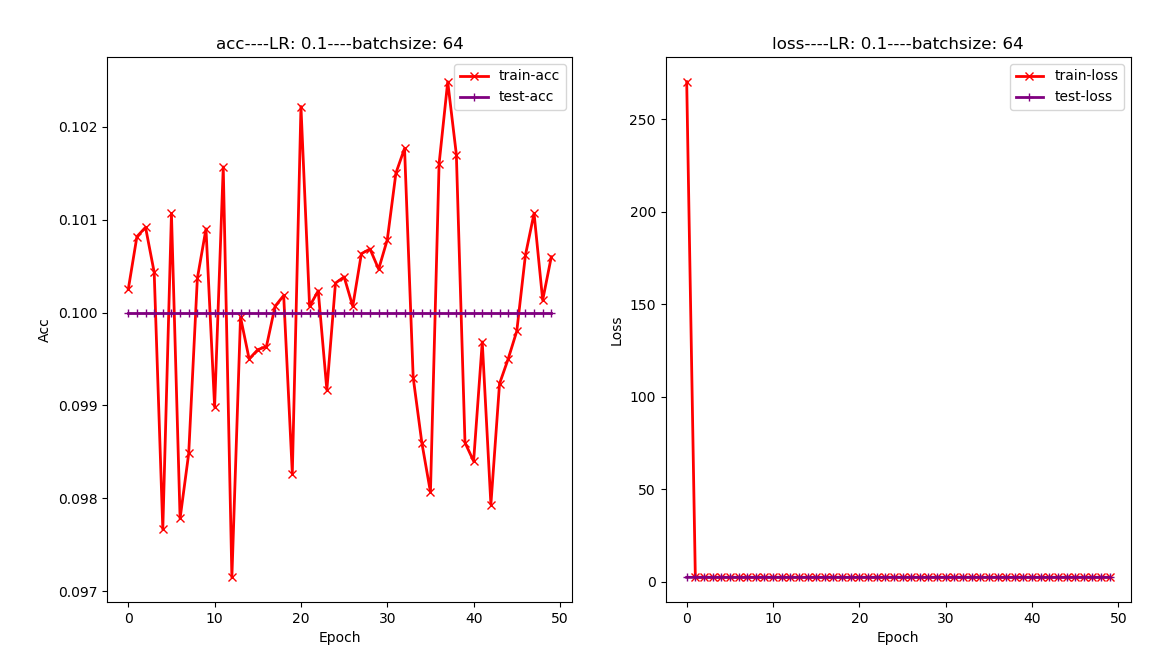
\includegraphics[width=2.7in]{./images/fashion3-1.png}
				%\caption{fig1}
			\end{minipage}%
		}%
		\subfigure[LR = 0.01]{
			\begin{minipage}[t]{0.5\linewidth}
				\centering
				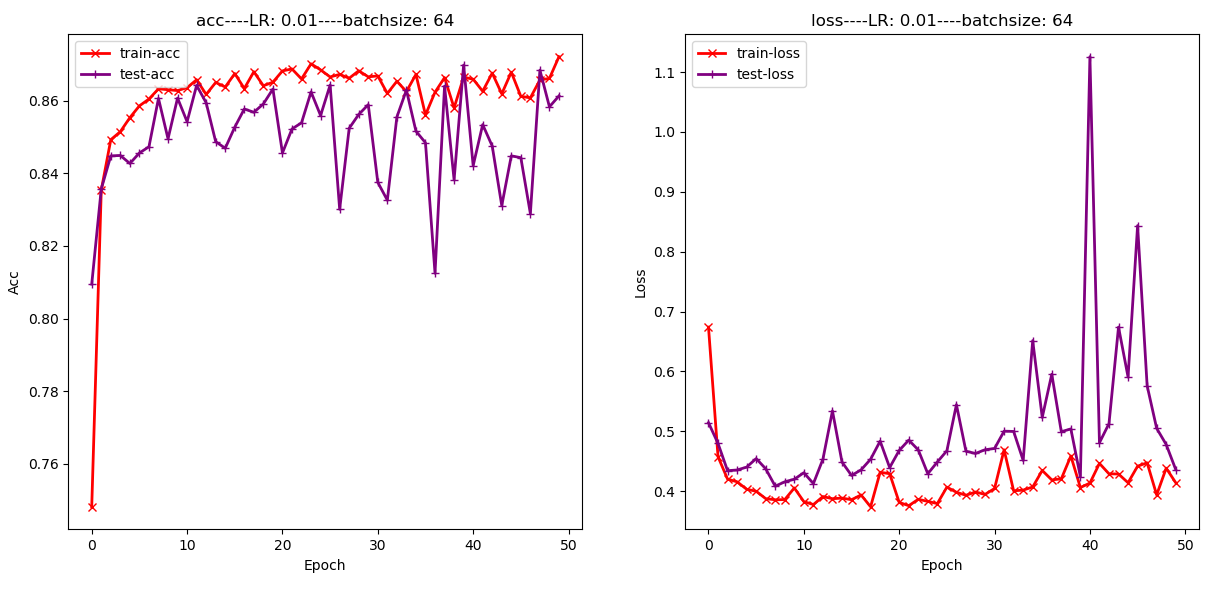
\includegraphics[width=3in]{./images/fashion3-2.png}
				%\caption{fig2}
			\end{minipage}%
		}
	
		\centering
		\subfigure[LR = 0.001]{
			\begin{minipage}[t]{0.5\linewidth}
				\centering
				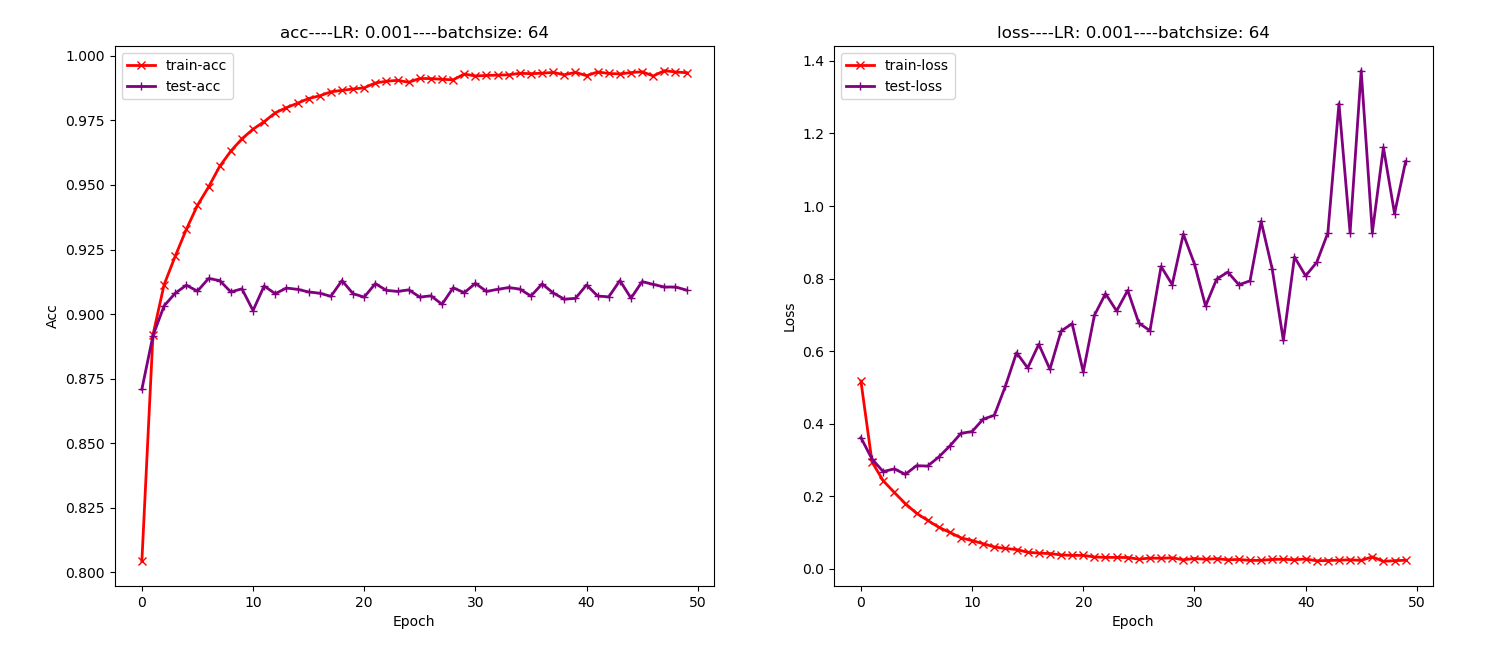
\includegraphics[width=3.2in]{./images/fashion3-3.png}
				%\caption{fig1}
			\end{minipage}%
		}%
		\subfigure[LR = 0.0001]{
			\begin{minipage}[t]{0.5\linewidth}
				\centering
				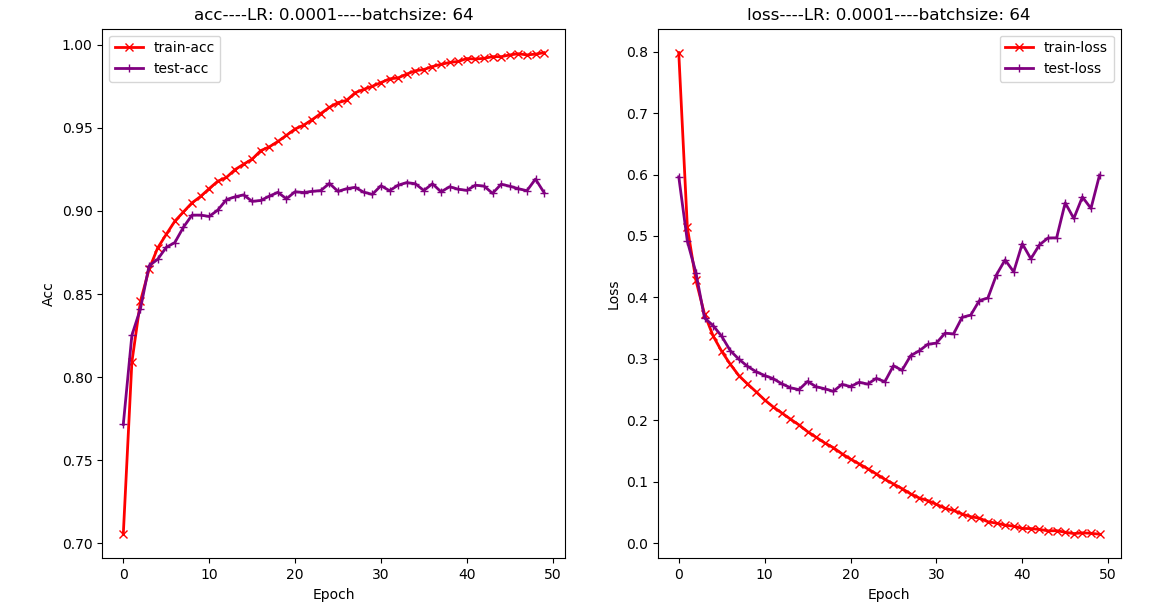
\includegraphics[width=2.7in]{./images/fashion3-4.png}
				%\caption{fig2}
			\end{minipage}%
		}
		\centering
		\caption{训练结果对比}
	\end{figure}
	
	LR = 0.0001 时的混淆矩阵如下:
	
	\begin{figure}[H]
		\centering
		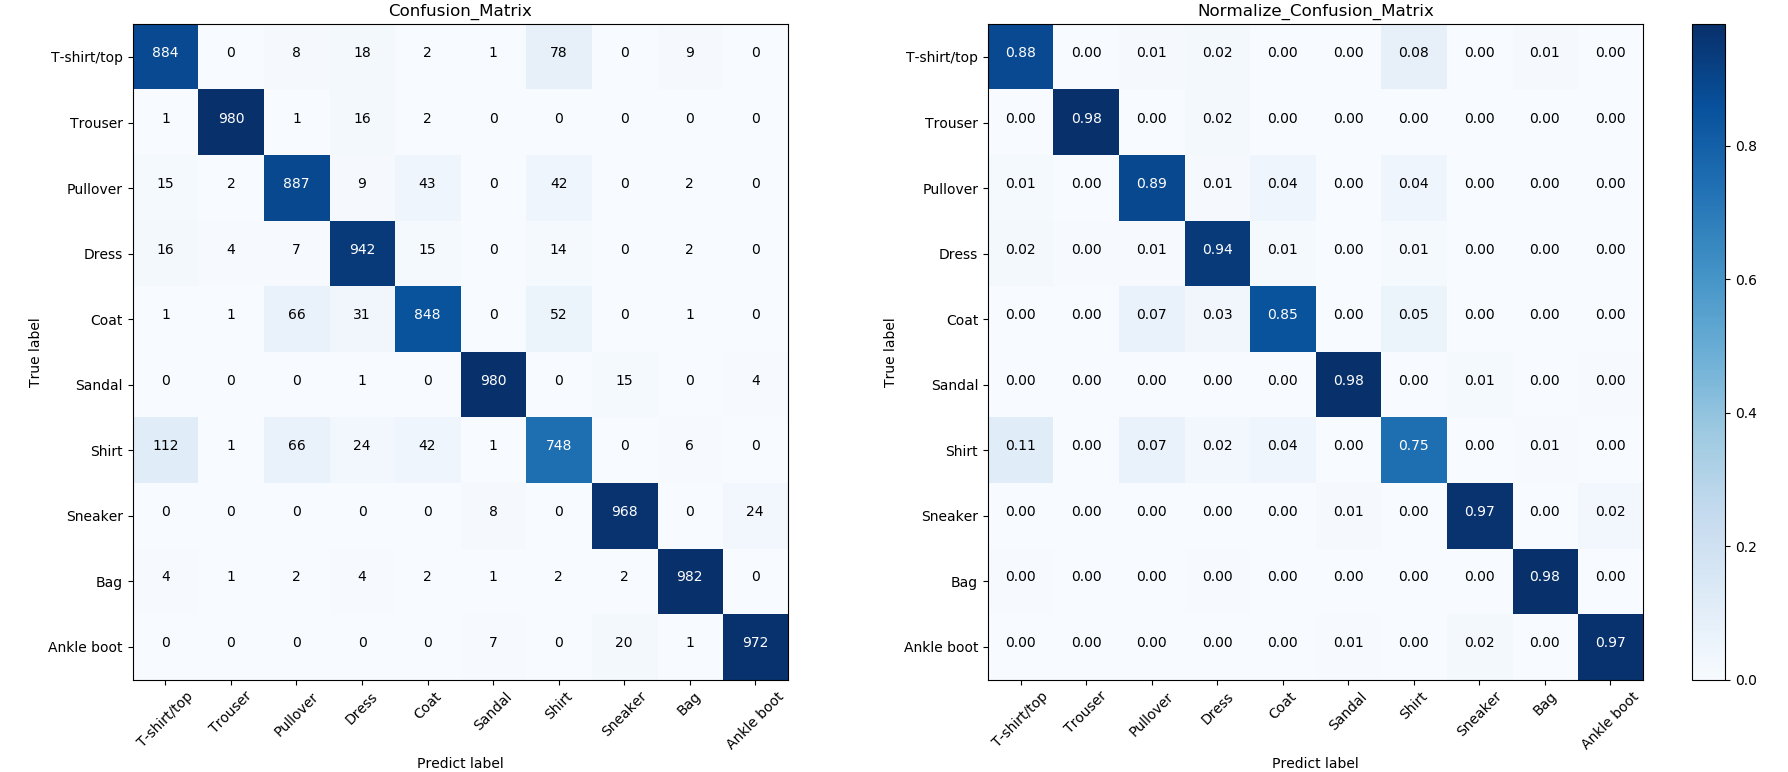
\includegraphics[width=5.5in]{./images/fashion4.png}
		\centering
		\caption{混淆矩阵}
	\end{figure}


	选取分类错误案例进行查看。
	
	\begin{figure}[H]
		\centering
		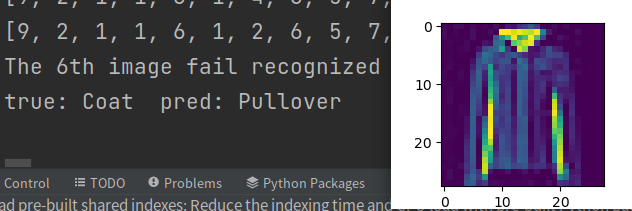
\includegraphics[width=4in]{./images/fashion5.png}
		\centering
		\caption{分类错误案例}
	\end{figure}
	
	网络将 coat(外套) 识别成了 pullover(套头衫),这两件物体的相似度即使是人眼也不一定可以分辨,这是可以理解的。


	\section{实验总结与结课感想}
	
	\subsection{实验总结}
	本次实验是应用神经网络学习方法进行分类的入门练习,完成三个实验后,总体而言,对神经网络的原理有了更深刻的认识,并对深度学习的代码框架也有了一定的了解。
	
	影响网络性能的参数太多,除了网络结构,优化器、学习率、样本训练批大小的参数调整都至关重要,有时仅仅是超参数不好,一个网络便无法起作用。例如在 MNIST 数据集中,当学习率为 0.1 时,网络的作用聊胜于无,相当于随机分类,调整学习率后效果可喜,同时,动态的学习率调整比固定学习率更加灵活,能快速收敛并减轻稳态震荡。除了网络结构的设计,神经网络的调参技巧也是同样需要大量的学习和经验积累的。
	
	\subsection{结课感想}
	
	记得这门课刚开始时老师花了很多篇幅在讲函数拟合,现在仔细体会,从 low-level 的像素级图像插值应用于图像融合和变形,到 high-level 的三维重建、物体识别,包括机器学习方法的本质全部都是函数拟合。在后段的课程了解到了很多图像处理的前沿知识,指针式的知识引导非常的高效。十分感谢刘老师,这门课程让我对图像理解有了近乎全新的认识。我是非数学系的学生,这门课程中老师对数学知识的组织和见解,让我受益匪浅,从开课到结束,听课都酣畅淋漓\footnote{本科的时候没去上刘老师的课太遗憾了哈哈。}。 \\
	
	课程作业代码:https://github.com/speedzjy/2021-DIP 
	
	\begin{thebibliography}{99}
		[1]PyTorch 官网 https://pytorch.org/ \\
		
		[2]Fashion-MNIST 数据集 https://github.com/zalandoresearch/fashion-mnist
		
	\end{thebibliography}
\end{document}

